\documentclass{llncs}
\usepackage{graphicx}

\begin{document}
% Adicionado para por apenas os numeros sem headers
\pagestyle{myheadings}
\title{Development of text-mining solutions to facilitate lipid metabolism interpretation in Genome-Scale Metabolic Models}

\author{Adriano Silva\inst{1,2}\and
Emanuel Cunha\inst{1,2} \and
João Capela\inst{1,2}}

\institute{Centro de Engenharia Biológica, Universidade do Minho, 4710-057 Braga, Portugal \and
LABBELS – Laboratório Associado, Braga, Guimarães, Portugal}
%
\maketitle              % typeset the header of the contribution
%
\begin{abstract}
Systems Biology is gaining importance in the unveil of cellular secrets. More precisely GSM models allow the contextualization of omic data and the progress of genomic engineering.
Still, the lack of macromolecule structural defined representation, such as lipids, is glaring.

-- Generic and defined duality

-- Resolution

\keywords{Genome-Scale Metabolic Models  \and Lipids representation.}
\end{abstract}
%
%
%
\section{Introduction}
\subsection{Context and motivation}
In the past two decades, Systems Biology has emerged as a discipline capable of integrating molecular knowledge into an understanding at a system level.
Biological systems are complex and oftentimes present non-linear relationships between their components. Accordingly, it is often resorted to mathematical models to understand and contextualize both each component separately and the system as a whole.
Genome-scale metabolic (GSM) models are useful tools that integrate genomic, biochemical, and physiological knowledge to better understand living organisms' metabolic behaviour \cite{Zou2018,Tavassoly2018}. 
These approaches can guide strain optimization and the production of a compound with industrial interest, such as lipidic biofuels produced by optimized yeasts and microalgae \cite{Sawangkeaw2013}.

The reconstruction of GSM models is gaining importance, mainly impulsed by the advances and cost-effectiveness of high-throughput technologies.
Over 6000 GSM models were reconstructed \cite{Gu2019} since the first model was published in 1999 \cite{Edwards1999}.
Nonetheless, the pace of reconstruction cannot keep up with the advancements of high-throughput technologies and, consequently, the generation of \textit{omics} data \cite{Kim2012}. The lack of integration of new data into GSM models is a problem inherent to this growth discrepancy.

Besides the usefulness of these models, their reconstruction is limited to the biochemical data existent in the available databases.
More precisely, complex macromolecules such as lipids and carbohydrates are often represented in their generic version, not providing the whole biochemical and structural information \cite{Gu2019}.
Particularly in the case of lipids, only a small number of reconstructed GSM models have structurally defined lipids with no or few relevant cross-references \cite{Capela}. 

Molecular structures are important to reliably integrate and annotate models' information regarding the different structurally defined lipid species.
The integration of lipid molecular information can be performed by taking advantage of the  \emph{de facto} lipid databases such as SWISS LIPIDS \cite{Aimo2015} and LIPID MAPS \cite{Sud2007}.
A tool capable of annotating and linking the different lipid species represented in GSM models with those databases could improve models' interpretability and accuracy. Consequently, such improvement could leverage the yield optimisation of lipidic biofuels \cite{Sawangkeaw2013}.




\subsection{Objective}

The main objective of this project is to integrate synonyms and abbreviations of lipids from SWISS LIPIDS and LIPID MAPS into a graph-based database. Then, those synonyms and abbreviations will be used to link GSM models' lipids with their molecular structures.

\section{State of art}
\subsection{Genome Scale Metabolic Models}
GSM models are computational tools that conjugate biochemical and genomic data of an organism, with the capacity to perform \emph{in silico} predictions of its phenotype under specific environmental and genetic conditions \cite{Rocha2007,Zhou2021}.

Thus, these models are key to the contextualization of high-throughput data and helpful in many other applications such as metabolic engineering, production of biochemicals and bio-materials, prediction of enzyme functions, or even in the discovery of drug targets \cite{Gu2019,Kim2017}.
Therefore, it is important to integrate reliable biochemical data into the reconstruction of these models to ensure their accuracy and further unequivocal interpretation \cite{Moseley2021,Passi2021}. 


\subsection{Lipid computational representation}
Lipids are macromolecules grouped into different classes according to their structural composition. 
They are composed of two biochemical components, the \textit{backbone}, usually composed of polar groups, and the \textit{sidechains} composed of apolar carbon linked chains.  
The differences in lipid structural polarity confer amphipathic characteristics to this macromolecule \cite{Fahy2011}. 
This means that in a hydrophilic environment the polar part of the molecule is attracted and the apolar one repelled.
This allows the generation of micelles, which are important for lipids' biological roles such as energy storage, signalling molecules, and being the main cell membrane components \cite{Cullis1986}.

As represented in Fig.\ref{fig1}, lipid structures can be split into two different parts: the backbone and the sidechains. The former is not variable for the whole class, remaining the same to the whole structurally defined lipids of the same class.
As for the sidechains, their structure can vary in the number of double bonds, stereochemistry and length.

According to Fahy and collaborators \cite{Fahy2009}, lipids can be divided into eight main classes: Fatty acyls,  Glycerolipids, Glycerophospholipids, Sphingolipids, Sterol Lipids, Prenol Lipids, Saccharolipids, and Polyketides. 
Due to the myriad of sidechains combinations, it is not possible to estimate how many distinct lipids can occur in nature \cite{Gyamfi2018,Capela}.

\begin{figure}
    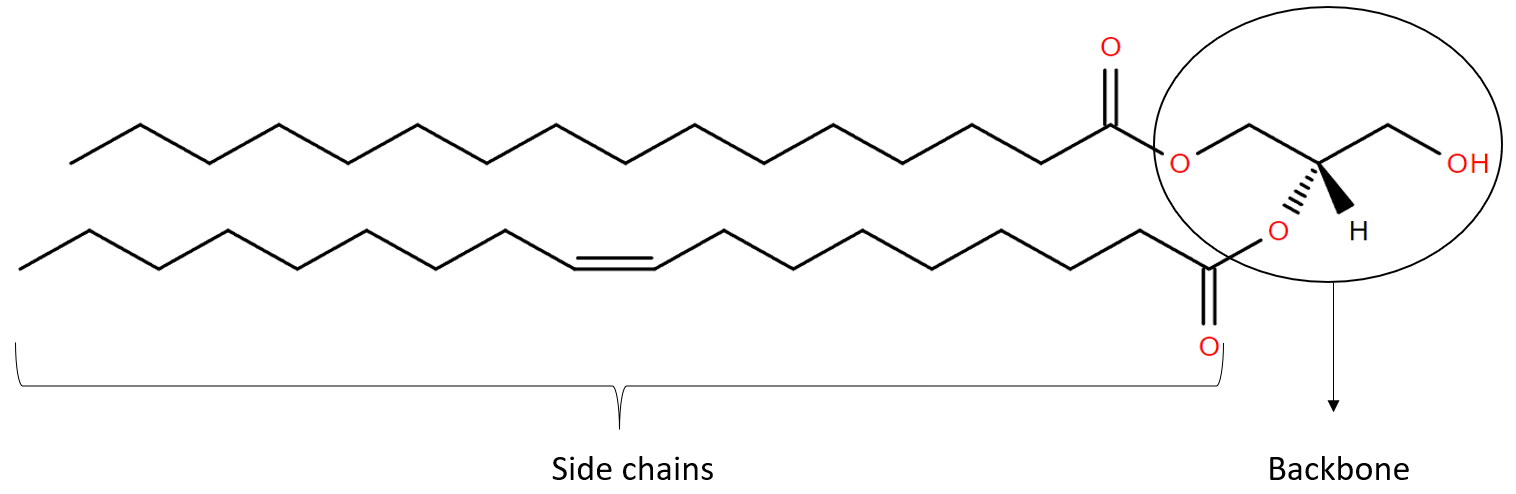
\includegraphics[width=\textwidth]{imagens/lipido.png}
    \caption{Representation of 1-hexadecanoyl-2-(9Z-octadecenoyl)-sn-glycerol structure extracted from LIPID MAPS. The backbone is the hydrophilic part of the lipid while the sidechains confer hydrophobicity.} \label{fig1}
\end{figure}

The growing importance of this macromolecule in health research and industrial applications brings the need to characterize their metabolic network and roles in cells.
Due to the immense amount of reactions, complex lipid biosynthetic pathways, and their inherent combinatorial complexity, it is almost impossible to study them by means of classical molecular biology \cite{Schutzhold}.

Computational approaches and, particularly, GSM models are helping to disentangle these issues \cite{Schutzhold}, however, lipid representation in such models is still not as trivial as desirable.
Despite the existence of lipid databases with defined structures, GSM models still fail to represent lipids with their structure completely defined \cite{Aung2013}. Nevertheless, a growing number of models with structurally defined lipids start to appear (see http://bigg.ucsd.edu/models), however, they still lack cross-references for lipid-specific databases, such as LIPID MAPS and SwissLipids. Such fact creates a gap between GSM models and \textit{de facto} lipid databases, hindering their interpretation and integration into other databases.


\subsection{Generic Representation in GSM models}
The metabolites and reactions present in GSM models highly depend on their source. As most databases (e.g., KEGG and MetaCyc) do not represent lipids as structurally defined, the absence of completely defined structures is propagated to those models, as can be seen in Fig.\ref{fig2}. 
This representation neglects the fact that sidechains are important components in the lipid metabolic network \cite{Schutzhold,Aung2013,Sanchez2019}.

\begin{figure}
    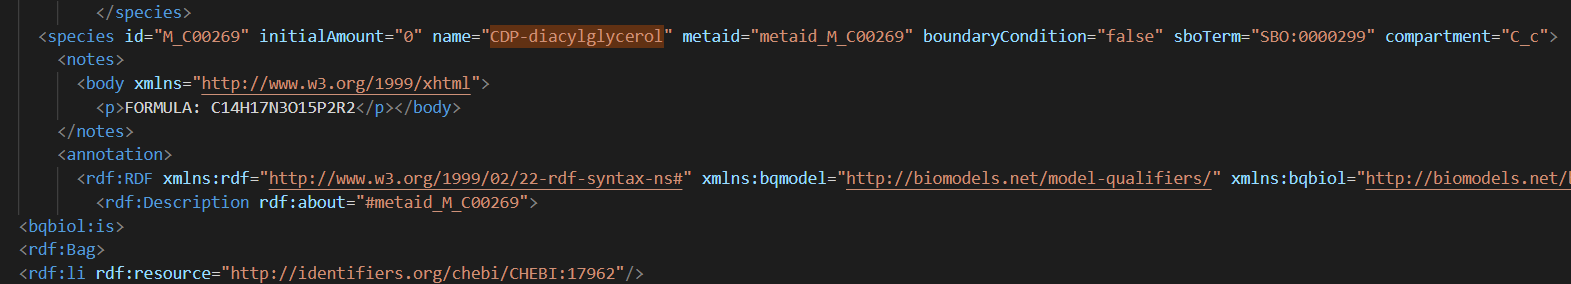
\includegraphics[width=\textwidth]{imagens/generica.png}
    \caption{Lipidic generic representation highlighted in \textit{Tgondii} model \cite{Tymoshenko2015}.  } \label{fig2}
\end{figure}

Accordingly, biosynthetic pathways are represented in generic terms, with generic lipids as reactants and products.
Based on this, we cannot access the exact lipids used in an hypothetic biosynthetic network.
Besides that, an abstract representation is linked to the loss of specificity of individual reactions \cite{Aung2013,Capela}.


Interestingly, we can still see the presence of cross-references to databases with the structure of these macromolecules. However, the same structure represents a multitude of structurally defined lipids of the class being represented. In these models, the name of the lipids is defined as the name of the class being represented, which, in most cases, only includes the name of the backbone, as can be seen in Fig.\ref{fig2}.

\subsection{Structurally defined representation in GSM models}
In the GSM models that comprise structurally defined lipids, the lipid name includes both the sidechains and the backbone. The sidechains' name is defined by the number of carbons followed by the number and the location of double bonds as well as their stereochemistry (Fig. \ref{fig3}).

\begin{figure}
    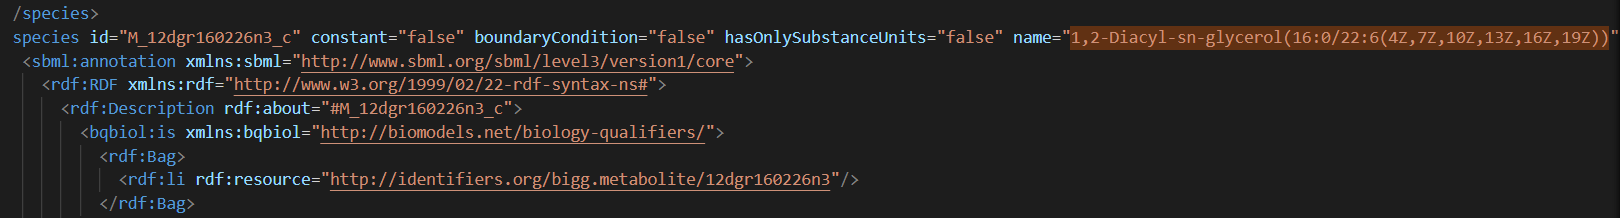
\includegraphics[width=\textwidth]{imagens/defenido.png}
    \caption{Lipidic defined representation highlighted in \textit{iLB1027-lipid} model \cite{Levering2016}.} \label{fig3}
\end{figure}

These approaches allow the generation of individual reactions with structurally defined lipids, in contrast with generic representations.
GSM models with defined lipids are could be more accurate, allowing the improvement of the flexibility, accuracy, and level of detail of these models. On the other hand, the inclusion of structurally defined versions of lipids can significantly increase the number of reactions in the model, which can be a drawback for some users \cite{Aung2013,Capela}.
Besides that, a lack of cross-references to \textit{de facto} lipid databases can be witnessed, which is not ideal for lipid structural confirmation, integration and interpretability.

\subsection{Lack of lipid annotations in GSM models}
 
Oppositely to GSM with lipidic generic representation, defined ones do not have an annotation to structure only to metabolites.
Overall, the use of lipid generic representations might not be appropriate in models aiming at lipid production optimization. 
However, defined representations usually lack in structural annotations, hindering their interpretation and curation.

\begin{figure}
    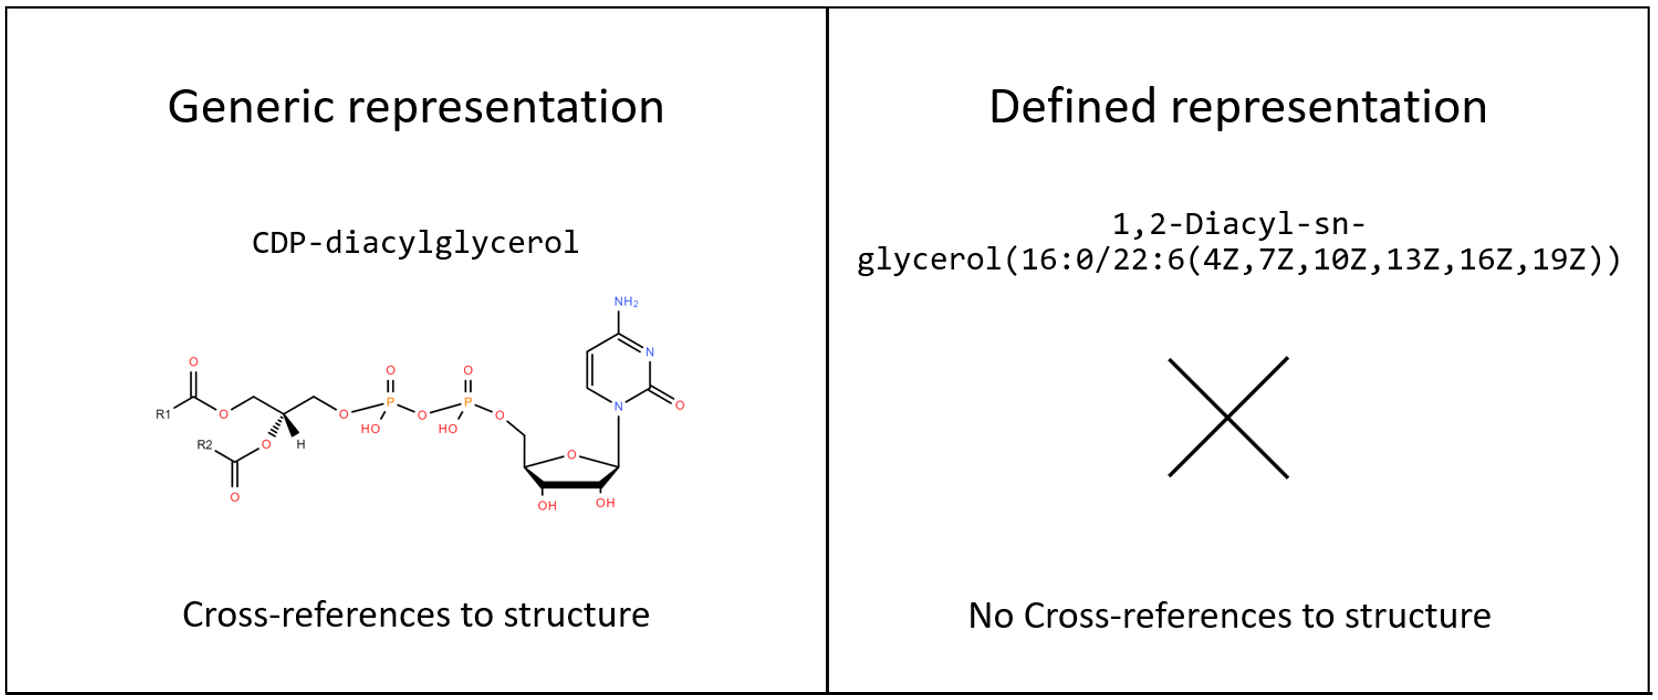
\includegraphics[width=\textwidth]{imagens/comparação.png}
    \caption{Comparation between generic and defined representations. First one extracted from the model \textit{Tgondii} \cite{Tymoshenko2015}, and second one from model \textit{iLB1027-lipid} \cite{Levering2016}. The structure from the generic lipid was extrated from LIPI MAPS.}
\end{figure}

A possible approach to fill this gap would be the integration of structural information in models. 
Such a solution would be achieved by the integration of synonyms and abbreviations, extracted from \textit{de facto} databases, as a link to the structural information. Those synonyms and abbreviations can be used to identify structurally defined lipids in the GSM models, as most of them provide a name or synonym, though not providing any cross-reference to other databases. 

\section{Methodology}

ETL is an integration data tool, that allows the gathering, processing, and integration of data, see Fig.\ref{fig4}. 
This is extremely useful in data cleaning and organization providing the bases for data analytics and machine learning approaches. 
Based on this, ETL pipelines could make easier the integration of structural information in our database.

\begin{figure}
    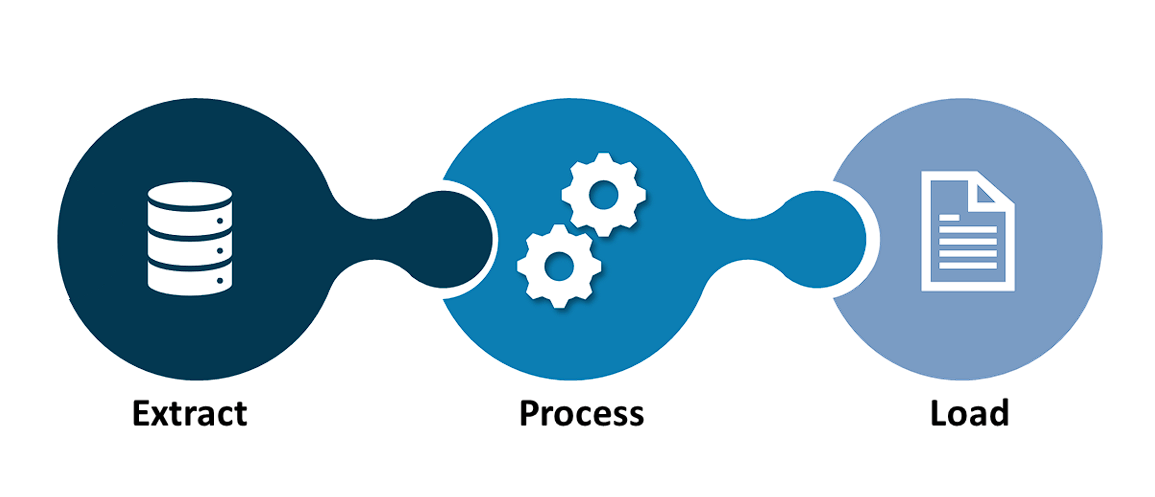
\includegraphics[width=\textwidth]{imagens/ETL.png}
    \caption{Escheme of the process done with ETL pipeline.
    First the ETL tool extracte data from multiple databases
    then processes all that data
    and finally integrates the data in our database.} \label{fig4}    
\end{figure}

Anotação de modelos:
    - match direto
    - decomposição do nome em dois (backbone e side chain) - queries à base de dados



\bibliographystyle{ieeetr}
\bibliography{referencias.bib}
\end{document}